\section{ACPOrderValidation}

Der \textit{ACP-Order-Validation}-Service bildet das Fundament für die Hauptfunktion des Admin-Clients -
dem Validieren von Bestellungen durch Einscannen des entsprechenden QR-Codes.

Hierfür wird ein Bearer-Token als Authorization-Parameter - gleich wie für die Verwendung des 
\nameref{clientfetchorderables} des Clients - benötigt.\\
Dieser wird mithilfe des \nameref{clientbearerauth}-Services, der aus dem Client übernommen worden ist,
generiert und setzt sich aus dem Namen und dem Passwort des angemeldeten ACP-Nutzers zusammen.

\subsection{Service-Routes}

\begin{code}[H]
    \centering
    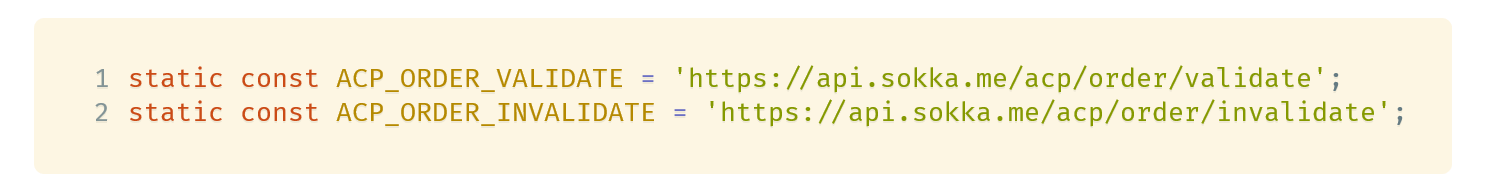
\includegraphics[width=1\textwidth]{images/Admin-Client/services/acpordervalidation/routes.png}
    \vspace{-25pt}
    \caption{API-Routes für den Order-Validation-Service}
\end{code}

\subsection{Validieren einer Bestellung}

Wird der QR-Code einer Bestellung mithilfe des Admin-Clients eingescanned, muss als erster Schritt dessen
Validität in Hinblick auf 

\begin{itemize}
    \item den Zeitpunkt der Bestellung (diese muss am Vortag vor der \glqq Closing Time\grqq\space aufgegeben worden sein)
    \item Zugehörigkeit der Bestellung zum eingeloggten Nutzer
    \item Gültigkeit des QR-Codes
\end{itemize}

überprüft werden.

Hierfür wird mit nachfolgend angeführter Funktion ein entsprechender Request nach dem Scan eines Codes
an die API gesendet.

\begin{code}[H]
    \centering
    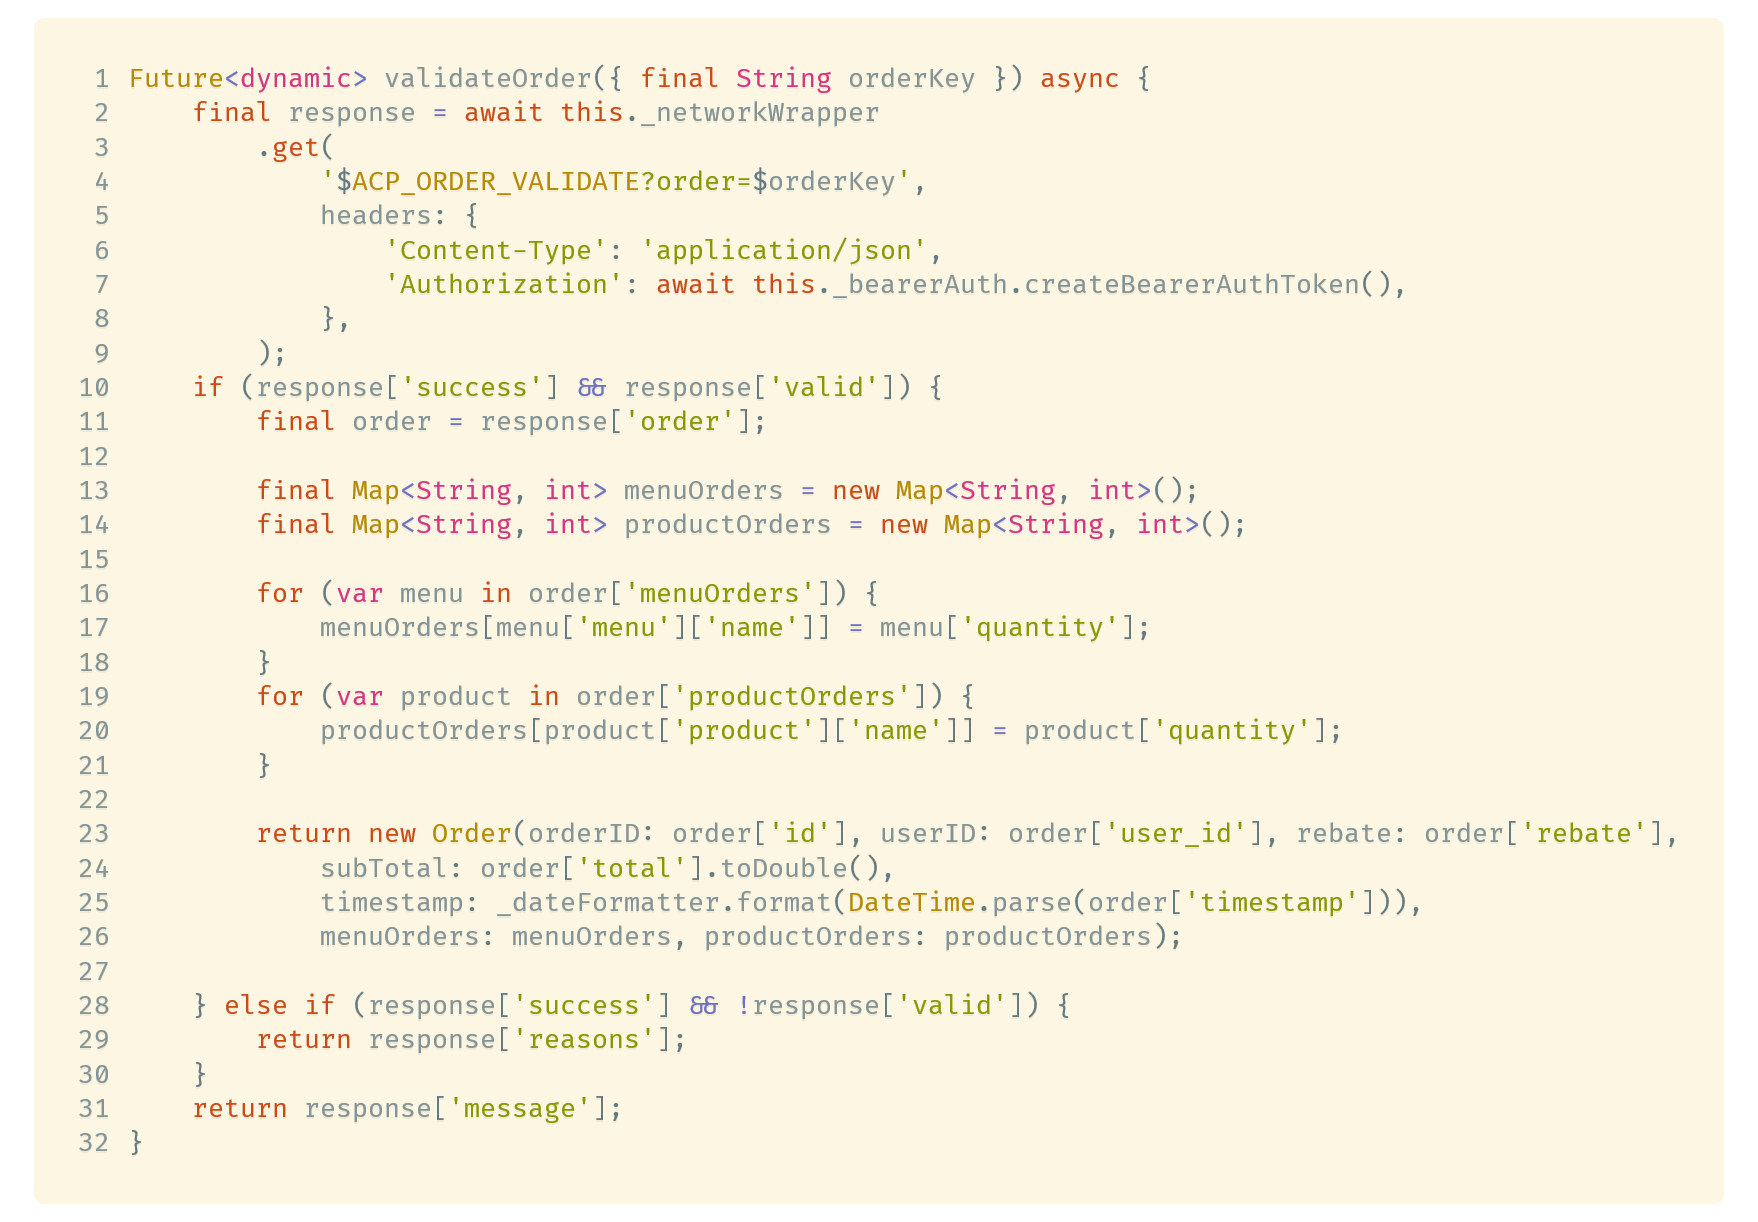
\includegraphics[width=1\textwidth]{images/Admin-Client/services/acpordervalidation/validateOrder.png}
    \vspace{-25pt}
    \caption{Überprüfen der Gültigkeit einer Bestellung}
\end{code}

Ist die Bestellung gültig und der Request damit erfolgreich, so werden die vom Nutzer bestellten
Waren, deren Preis, der Rabatt und der Gesamtpreis nach Abzug des Rabatts in einem Dialog-Fenster
angezeigt.

Das Personal kann nun den entsprechenden Betrag vom Nutzer kassieren und die Bestellung abschließen
und den QR-Code invalidieren.

\subsection{Abschließen einer Bestellung}

Wird eine Bestellung durch den Admin-Client als gültig erkannt und in weiterer Folge durch den
Restaurantangestellten kassiert muss die Bestellung und deren QR-Code ungültig gemacht werden,
um nicht mehrmals vorgezeigt werden zu können.

Dies kann über den Druck eines Buttons im oben erwähnten Dialog-Fenster, in dem die relevanten Daten
der Bestellung aufgelistet sind, durchgeführt werden.\\
Dabei wird folgende Anfrage an die API gesendet:

\begin{code}[H]
    \centering
    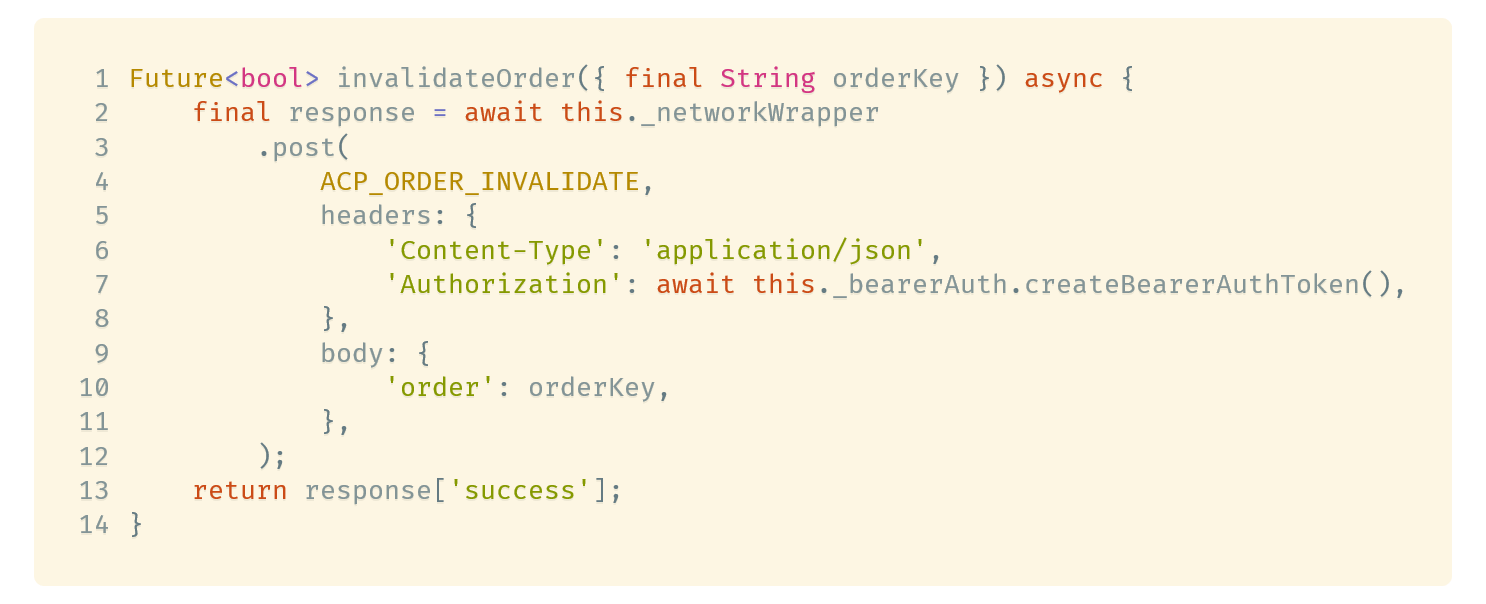
\includegraphics[width=1\textwidth]{images/Admin-Client/services/acpordervalidation/invalidateOrder.png}
    \vspace{-25pt}
    \caption{Invalidieren einer Bestellung}
\end{code}

